\tocsection{\textbf{9/14/26 Lecture 8}: Intro to the Lebesgue Integral}

First, we finish up the proof for Caratheodory's theorem seen above.\\

\begin{proof}{Proof of 4)}
    Let $\nu$ be a measure on $\sigma(\cal{A}_0)$ such that $\nu(A) = \ell(A)$ for all $A \in \cal{A_0}$. WE want to show that $\nu(A) = \mu^{*}(A)$ for all $A \in \sigma(A_n)$.\\

    First, we will consider the case when $\mu^{*}$ is finite. Fix $A \in \sigma(\cal{A}_0)$ and let $A \subseteq \bigcup_{n} A_n$ with $A_n \in \cal{A_0}$. Then, as 
    \[ \nu(A) \leq \sum_{n = 1}^{\infty} \nu(A_n) = \sum_{n = 1}^{\infty} \ell(A) \]
    taking infs over such covers, we see that $\nu(A) \leq \mu^{*}(A)$.\\

    Now, we want to show that $\nu$ and $\mu^{*}$ agree on sets of the form $\bigcup_{n} A_n$ for $A_n \in \cal{A}_0$. Let
    \[ B_n = \bigcup_{j = 1}^{n} A_j \]
    then, we see that
    \[ \mu^{*}(\cup_{i = 1}^{\infty} A_i) = \lim_{n \to \infty} \mu^{*}(B_n) = \lim_{n \to \infty} \nu(B_n) = \nu(\cup_{i = 1}^{\infty} A_i) \]
    Now, choose $A_n$ so that $A \subseteq \bigcup_{i = 1}^{\infty} A_n$ and $A_n \in \cal{A}_0$ such that $\mu^{*}(A) + \epsilon \geq \sum_{n} \mu^{*}(A_n)$. Then, 
    \begin{align*}
        \mu^{*}(A) + \epsilon &\geq \sum_{n} \mu^{*}(A_n)\\
        &\geq \mu^{*}\left(\bigcup_{i = 1}^{\infty} A_n\right)
    \end{align*}
    thus, we see that $\epsilon \geq \mu^{*}\left(\bigcup_{i = 1}^{\infty} A_n\right) - \mu^{*}(A) = \mu^{*}(\bigcup_{i = 1}^{\infty} A_n \backslash A)$ (this step requires that $\mu^{*}$ is finite). Then, we see that
    \begin{align*}
        \mu^{*}(A) \leq \mu^{*}(\bigcup_{i = 1}^{\infty} A_n) &= \nu(\bigcup_{i = 1}^{\infty} A_n)\\
        &= \nu(A) + \nu(\bigcup_{i = 1}^{\infty} A_n \backslash A)\\
        &\leq \nu(A) + \mu^{*}(\bigcup_{i =1}^{\infty} A_n \backslash A)\\
        &< \nu(A) + \epsilon
    \end{align*}
    where the second to last step came from above. Thus, $\mu^{*}(A) \leq \nu(A) + \epsilon$ for all $\epsilon$, so $\mu^{*}(A) \leq \nu(A)$.\\

    Now, if $\mu^{*}$ is $\sigma$-finite, then we can write $X = \bigcup_{n = 1}^{\infty} X_n$ with $X_n \uparrow X$ with $\mu^{*}(X_n) < \infty$. Then, if we consider the measures $\mu^{*}\res{X_n}$ and $\nu\res{X_n}$ (where $\mu\res{X_n}(A) = \mu(X_n \cap A)$), we see that as $\mu^{*}\res{X_n}$ and $\nu\res{X_n}$ are finite measures, they have to agree by the argument above. Then, for $A \in \sigma(\cal{A_0})$, we see that
    \[ \mu^{*}(A) = \lim_{n \to \infty} \mu^{*}(A \cap X_n) = \lim_{n \to \infty} \nu(A \cap X_n) = \nu(A) \]
    which was desired. 

    $\qed$
\end{proof}

Now, lets move on to functions. As a motivation, consider $C[0, 1]$ with the metric
\[ d(f, g) = \int_{0}^{1} \abs{f(x) - g(x)}dx \]
This is nice until you realize that it doesn't make $C[0, 1]$ complete! Consider the functions as described below

\begin{center}
    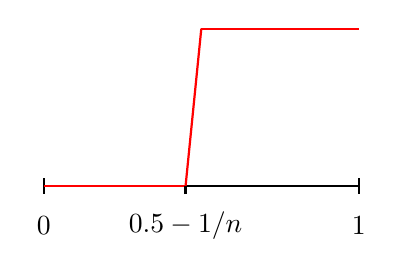
\begin{tikzpicture}
        \draw[thick] (-2, 0) -- (2, 0);
        \draw[thick] (-2, 0.1) -- (-2, -0.1);
        \draw[thick] (2, 0.1) -- (2, -0.1);


        \node at (-2, -0.5) {$0$};
        \node at (2, -0.5) {$1$};

        \draw[thick, red] (-2, 0) -- (-0.2, 0);
        \draw[thick, red] (-0.2, 0) -- (0, 2);
        \draw[thick, red] (0, 2) -- (2, 2);
        \node at (-0.2, -0.5) {$0.5 - 1/n$};
        \draw[thick] (-0.2, -0.1) -- (-0.2, 0);
    \end{tikzpicture}
\end{center}

These turn out to be Cauchy under this metric, but they converge to the function
\[ f(x) = \chi_{[1/2, 1]} \]
where $\chi_{A}$ is the characteristic function of $A$ which is $1$ on $A$ and $0$ off of $A$. The problem is that $\chi_{[1/2, 1]}$ is not continuous, so it cannot be the limit. This example is somewhat tame in that the limiting function is still Riemann integrable, but there are some Cauchy sequences in $C[0, 1]$ that converge to non Riemann integrable functions, so we want to see how to fix that.\\

First, consider $\chi_{\Q \cap [0, 1]}$. This is not Riemann integrable as $U(\chi_{\Q \cap [0, 1]}, P) = 1$ and $L(\chi_{\Q \cap [0, 1]}, P) = 0$ for any partition. However, maybe we should still try to make sense of it's integral.\\

\textbf{Question:} What should $\int \chi_{\Q \cap [0, 1]} dx$ be?

\textbf{Intuitive Answer} Since $\int$ is the area under a function, $\int \chi_{E}$ should be the measure of $E$ for any set $E$. That is, $\int \chi_{E} = \lambda(E)$. Then, as $\lambda(\Q \cap [0, 1]) = 0$, it would be natural to expect that $\int \chi_{\Q \cap [0, 1]} dx = 0$. How do we formalize this? First, we start by defining the integral on characteristic functions as we did above.\\

\begin{definition}[\textbf{Definition 8.1:} Lebesgue Integral of a Characteristic Function]
    Given a measure space $(X, \cal{A}, \mu)$, define the \emph{Lebesgue integral} of a characteristic function $\chi_{A}$ for $A \in \cal{A}$ to be
    \[ \int \chi_{A} d\mu = \mu(A) \]
\end{definition}

\begin{definition}[\textbf{Definition 8.2:} Simple Functions]
    A \emph{simple function} is a function of the form
    \[ f = \sum_{i = 1}^{\infty} c_n \chi_{A_n} \]
\end{definition}
Then, as we want our integral to be linear as well, we can define
\[ \int \sum_{n = 1}^{\infty} a_n \chi_{A_n} d\mu = \sum_{n = 1}^{\infty} a_n\mu(A_n) \]
for $A_n \in \cal{A}$.\\

Now, heres a definition that seems random right now, but we will soon see it describes exactly what we want.

\begin{definition}[\textbf{Definition 8.3:} Measurable Functions]
    A function $f : X \to \R$ is \emph{measurable} if $\{x \in X \col f(x) > a\} = f^{-1}(a, \infty) \in \cal{A}$ for all $a \in \R$.
\end{definition}

Now, we see, considering some $\chi_{A}$, that $f^{-1}(a, \infty) = \emptyset$ if $a \geq 1$, $f^{-1}(a, \infty) = A$ if $0 \leq a < 1$, and $f^{-1}{a, \infty} = X$ if $a < 0$. Thus, we see that $\chi_{A}$ is measurable if $A$ is a measurable set!